%!TEX root = ../MainDoc.tex
\newpage
\section{Class diagrams}
\label{classDiagrams}

\subsection{Package core}
\begin{figure}[H]
  %\caption{Class diagram of the package: \texttt{core}}
  \centering
    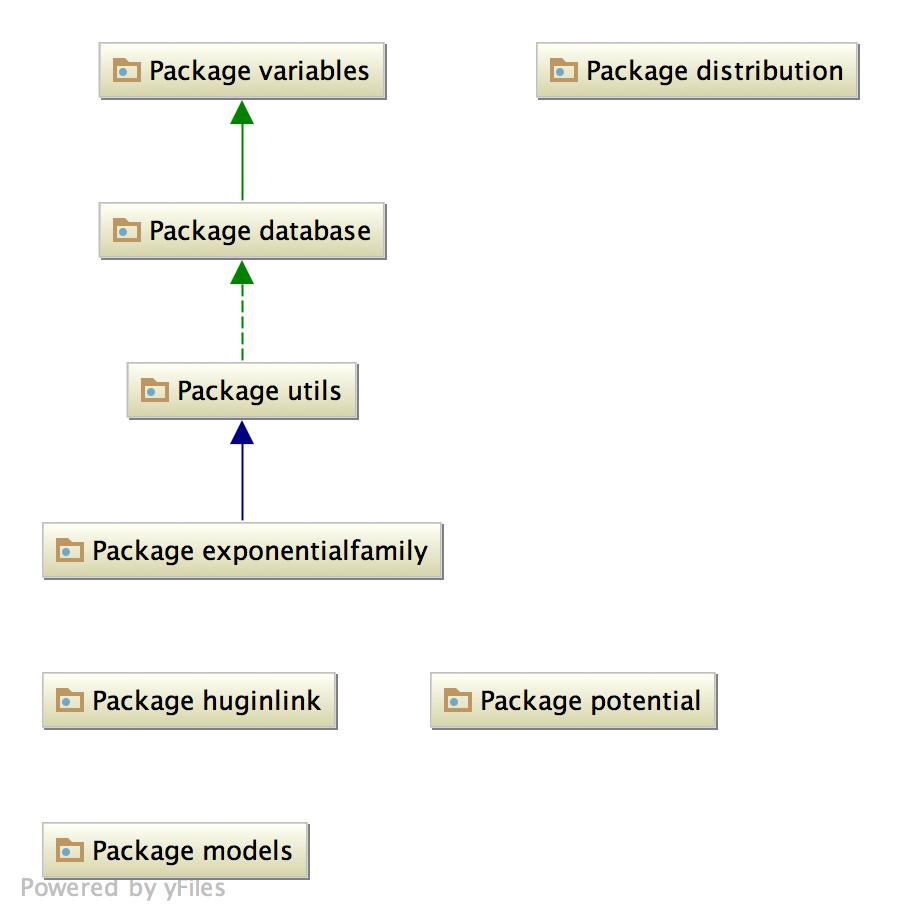
\includegraphics[width=0.5\textwidth]{ClassDiagrams/core.jpg}
\end{figure}

\subsection{Package core.database}
\begin{figure}[H]
  %\caption{Class diagram of the package: \texttt{core.database}}
  \centering
    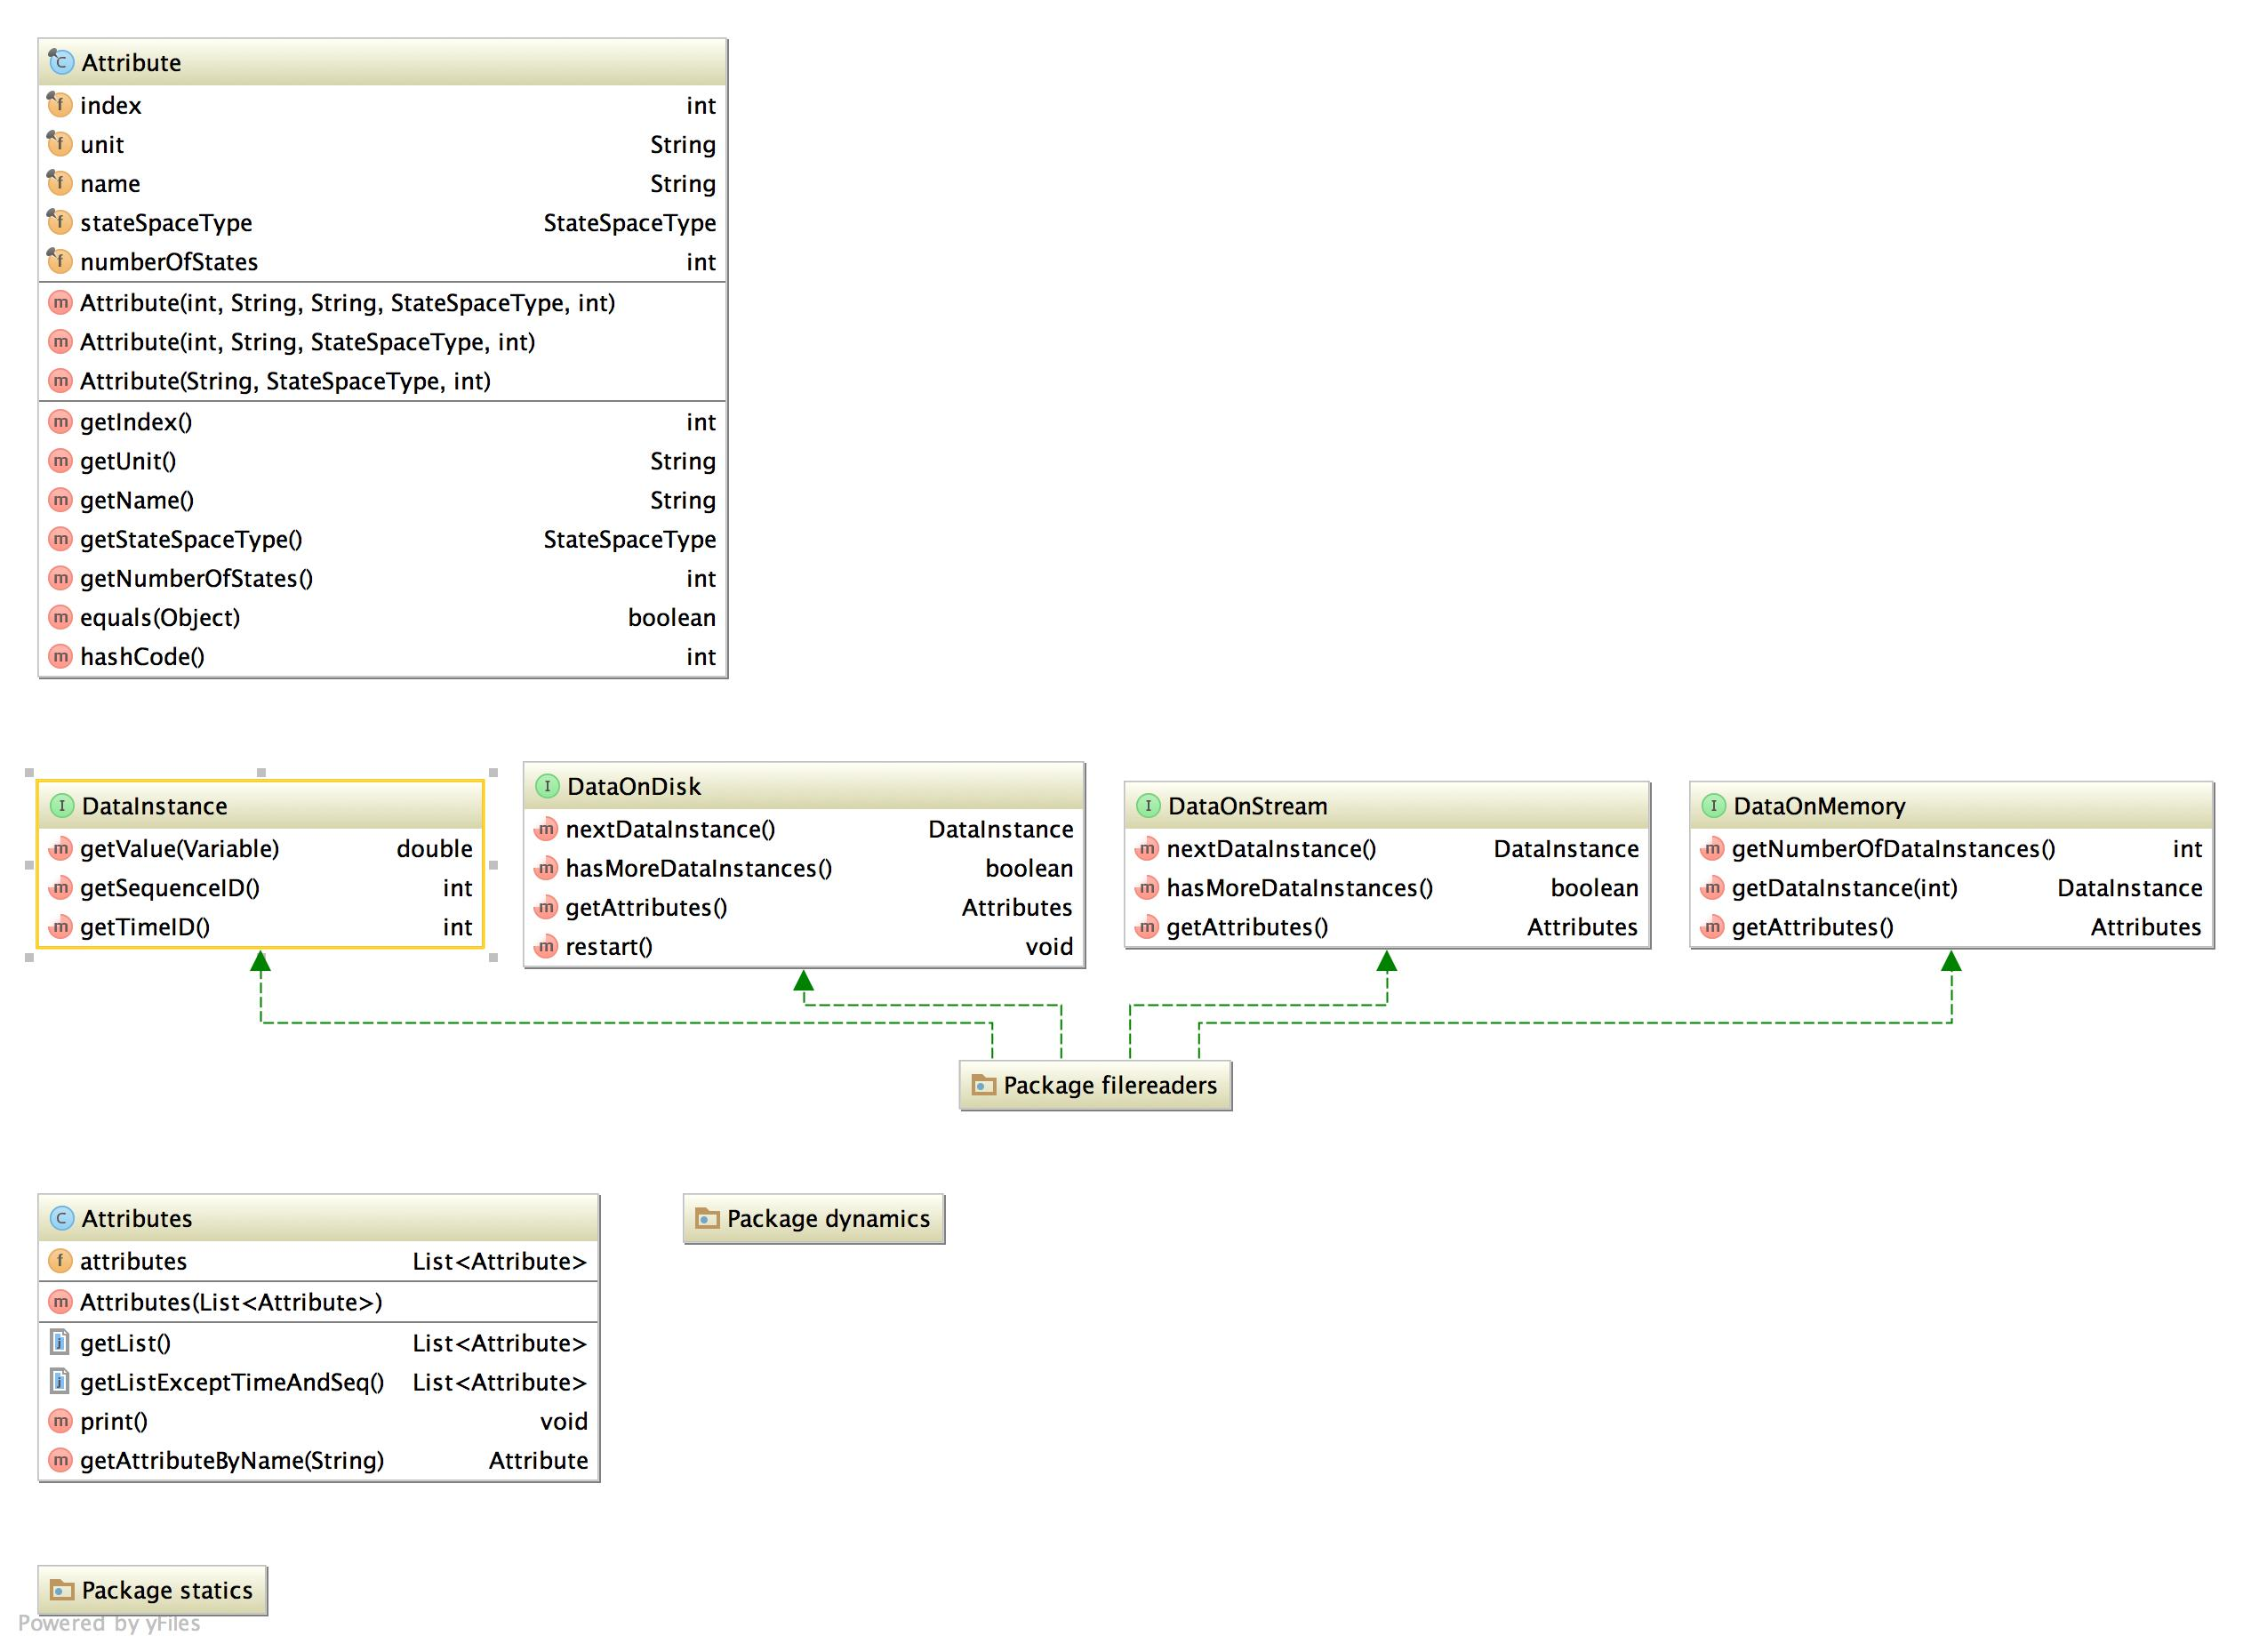
\includegraphics[width=\textwidth]{ClassDiagrams/core_database.jpg}
\end{figure}

\subsection{Package core.database.dynamics}
\begin{figure}[H]
  %\caption{Class diagram of the package: \texttt{core.database.dynamics}}
  \centering
    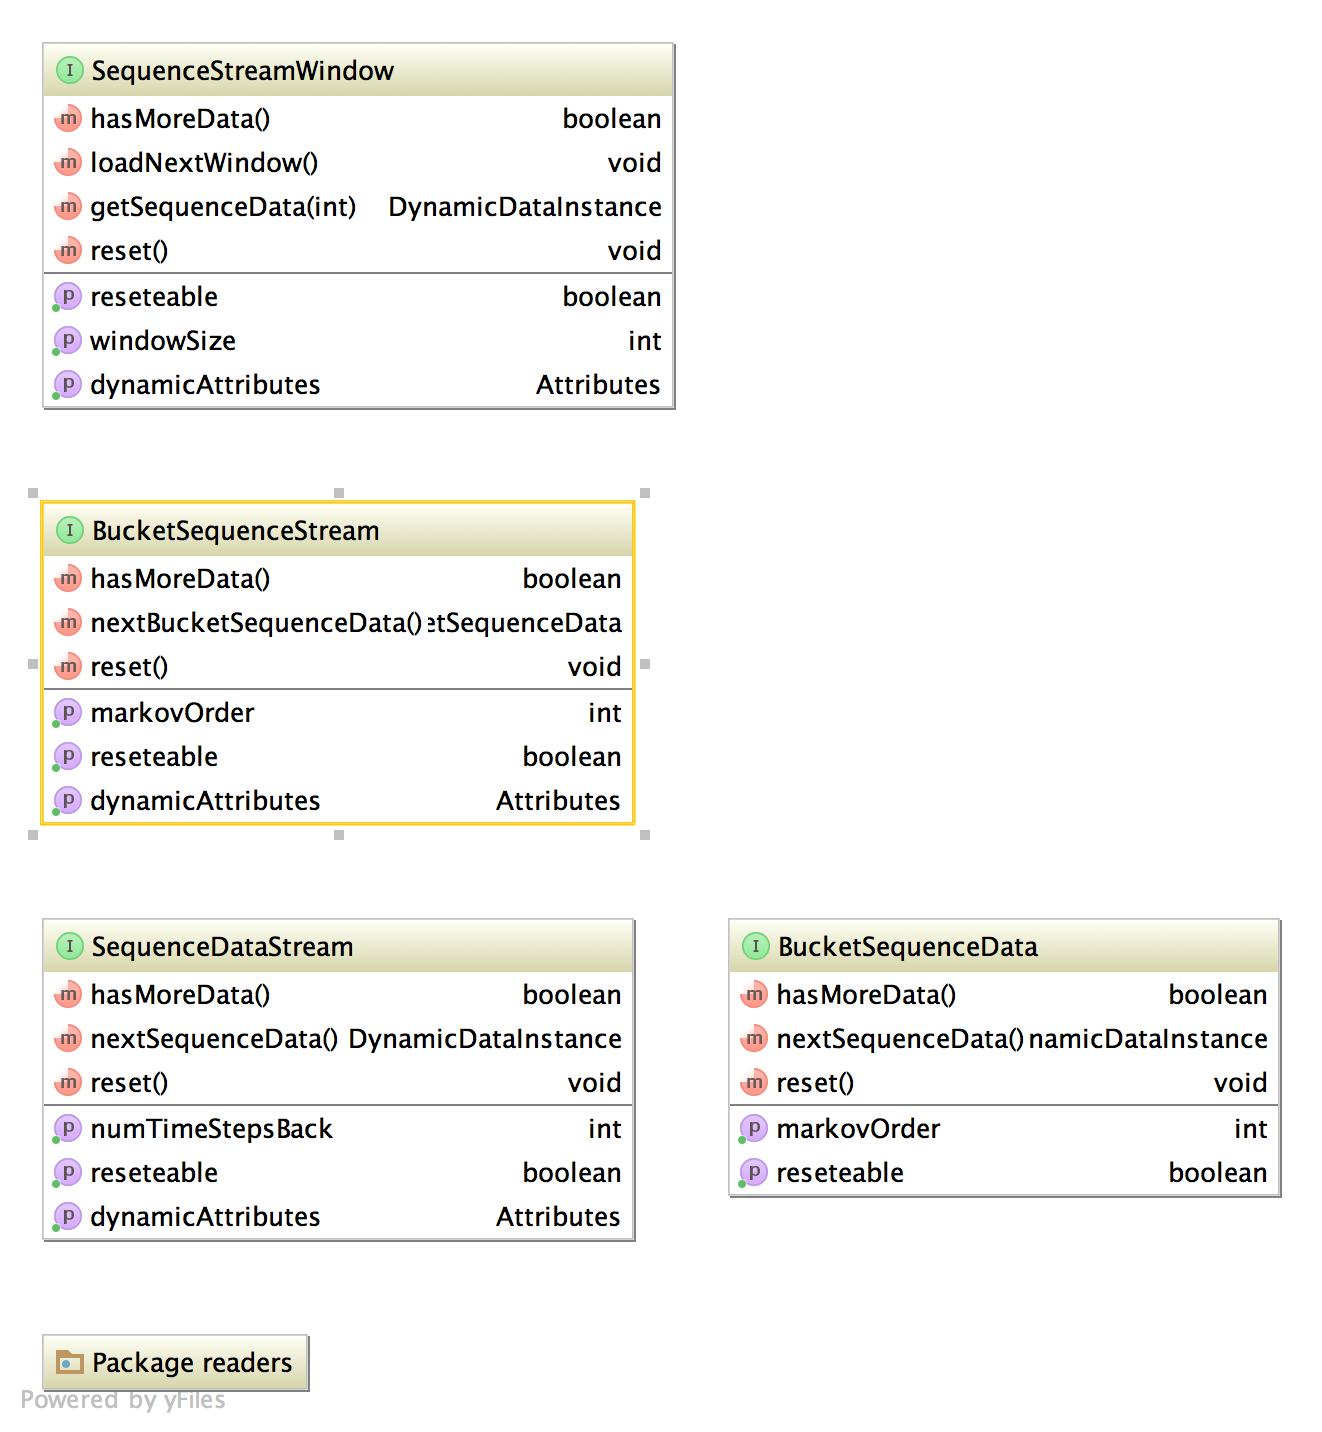
\includegraphics[width=0.7\textwidth]{ClassDiagrams/core_database_dynamics.jpg}
\end{figure}

\subsection{Package core.database.readers}
\begin{figure}[H]
  %\caption{Class diagram of the package: \texttt{core.database.dynamics.readers}}
  \centering
    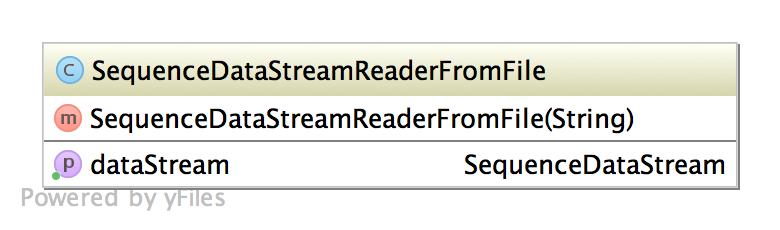
\includegraphics[width=0.4\textwidth]{ClassDiagrams/core_database_dynamics_readers.jpg}
\end{figure}

\subsection{Package core.database.filereaders}
\begin{figure}[H]
  %\caption{Class diagram of the package: \texttt{core.database.filereaders}}
  \centering
    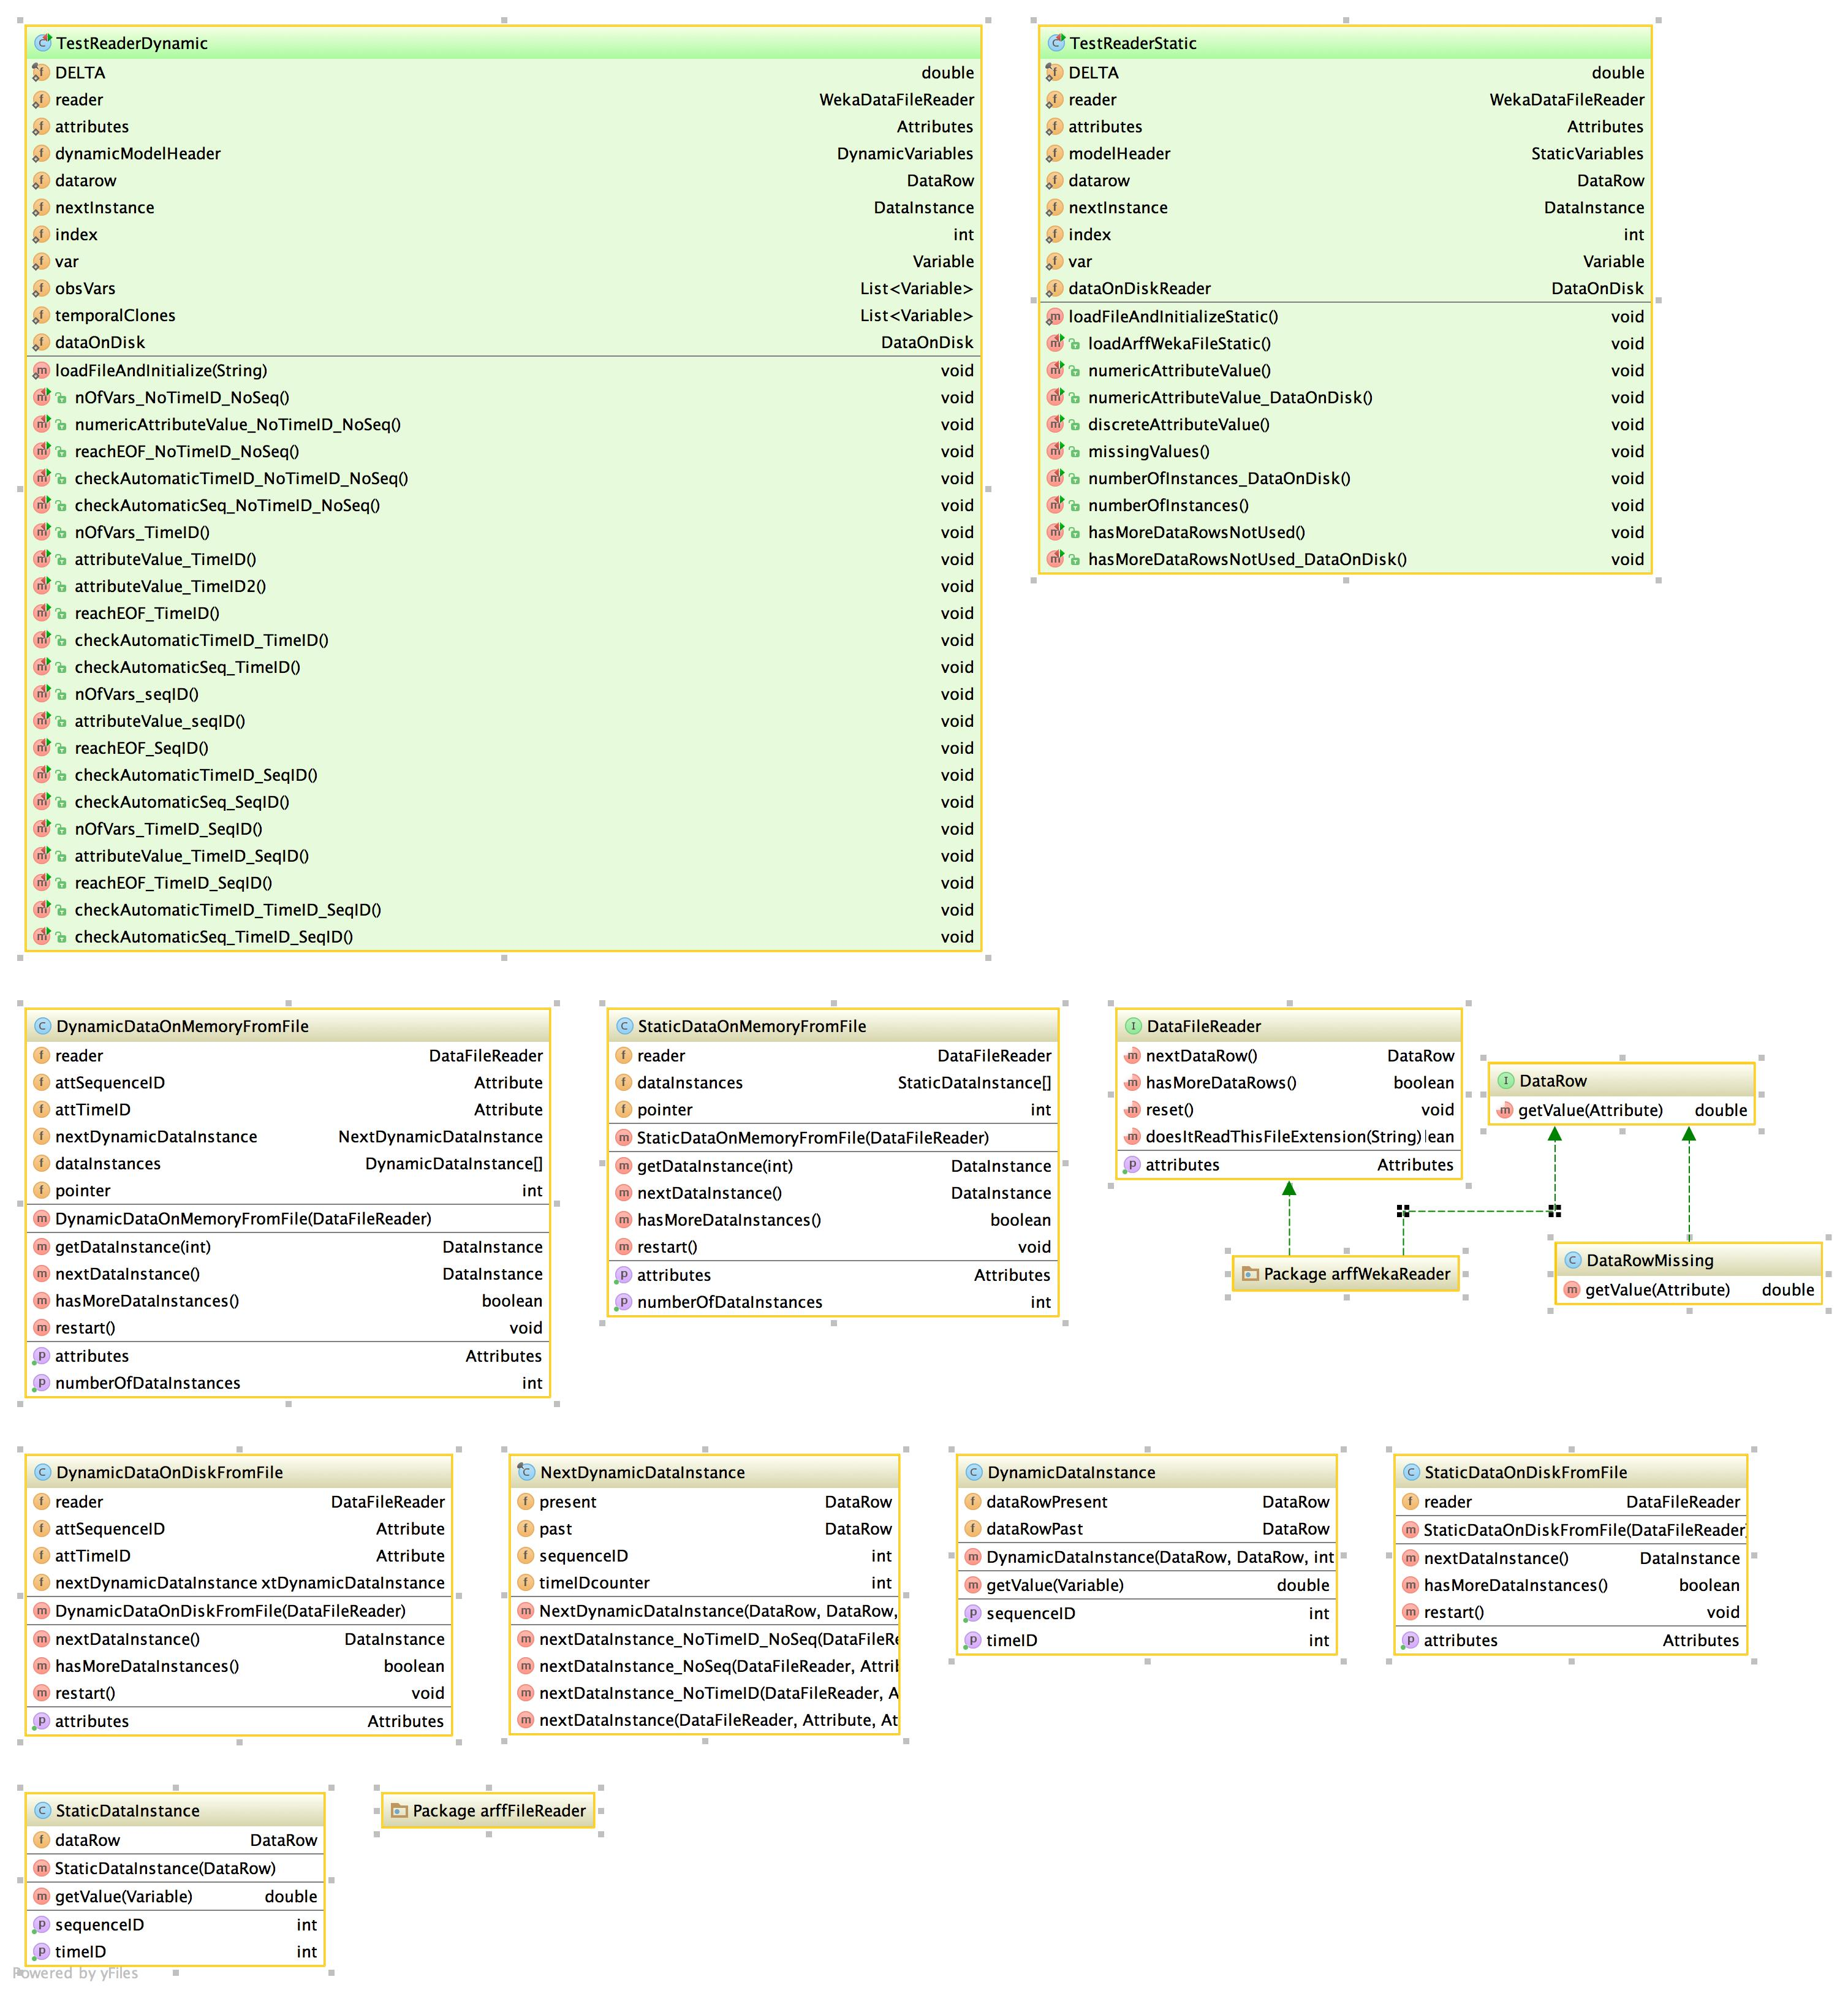
\includegraphics[width=\textwidth]{ClassDiagrams/core_database_filereaders.jpg}
\end{figure}

\subsection{Package core.database.arffFileReader}
\begin{figure}[H]
  %\caption{Class diagram of the package: \texttt{core.database.filereaders.arffFileReader}}
  \centering
    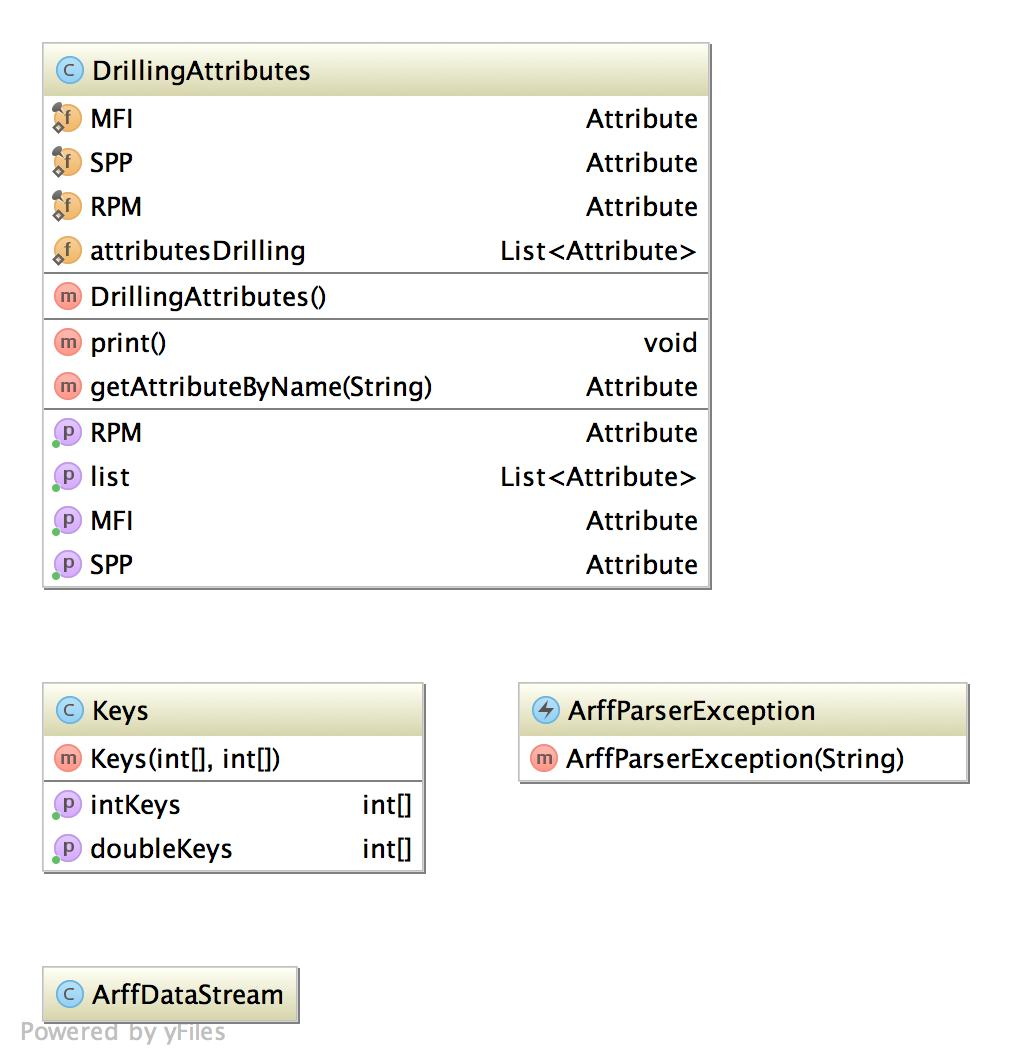
\includegraphics[width=0.5\textwidth]{ClassDiagrams/core_database_filereaders_arfffilereader.jpg}
\end{figure}


\subsection{Package core.database.arffWekaReader}
\begin{figure}[H]
  %\caption{Class diagram of the package: \texttt{core.database.filereaders.arffWekaReader}}
  \centering
    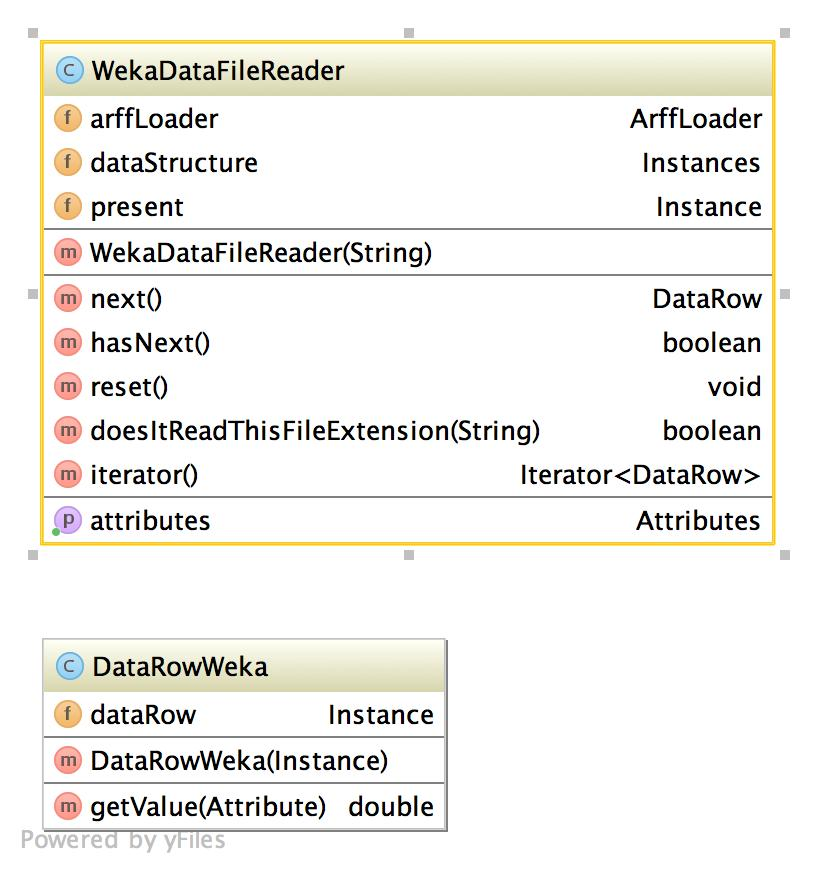
\includegraphics[width=0.5\textwidth]{ClassDiagrams/core_database_filereaders_arffwekareader.jpg}
\end{figure}

\subsection{Package core.distribution}
\begin{figure}[H]
  %\caption{Class diagram of the package: \texttt{core.distribution}}
  \centering
    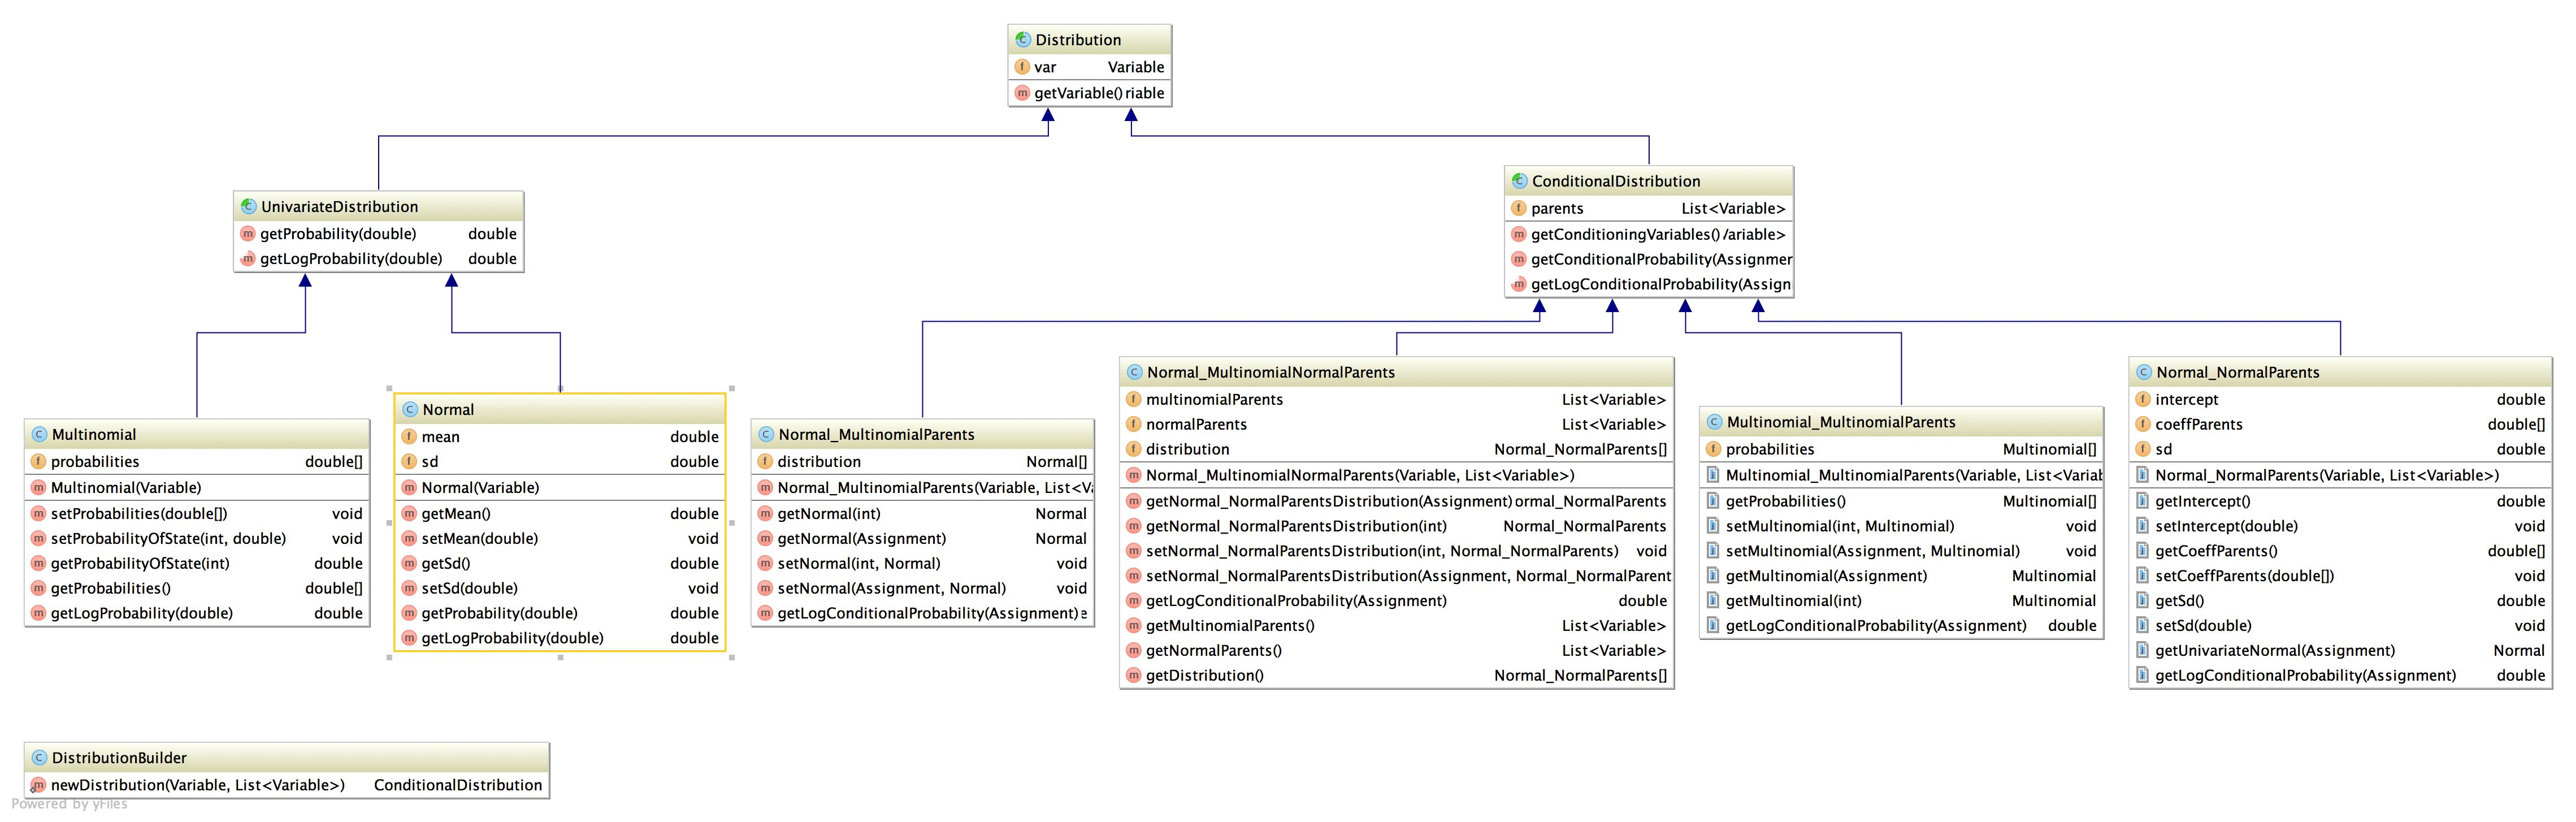
\includegraphics[width=\textwidth]{ClassDiagrams/core_distribution.jpg}
\end{figure}

\subsection{Package core.exponentialfamily}
\begin{figure}[H]
  %\caption{Class diagram of the package: \texttt{core.exponentialfamily}}
  \centering
    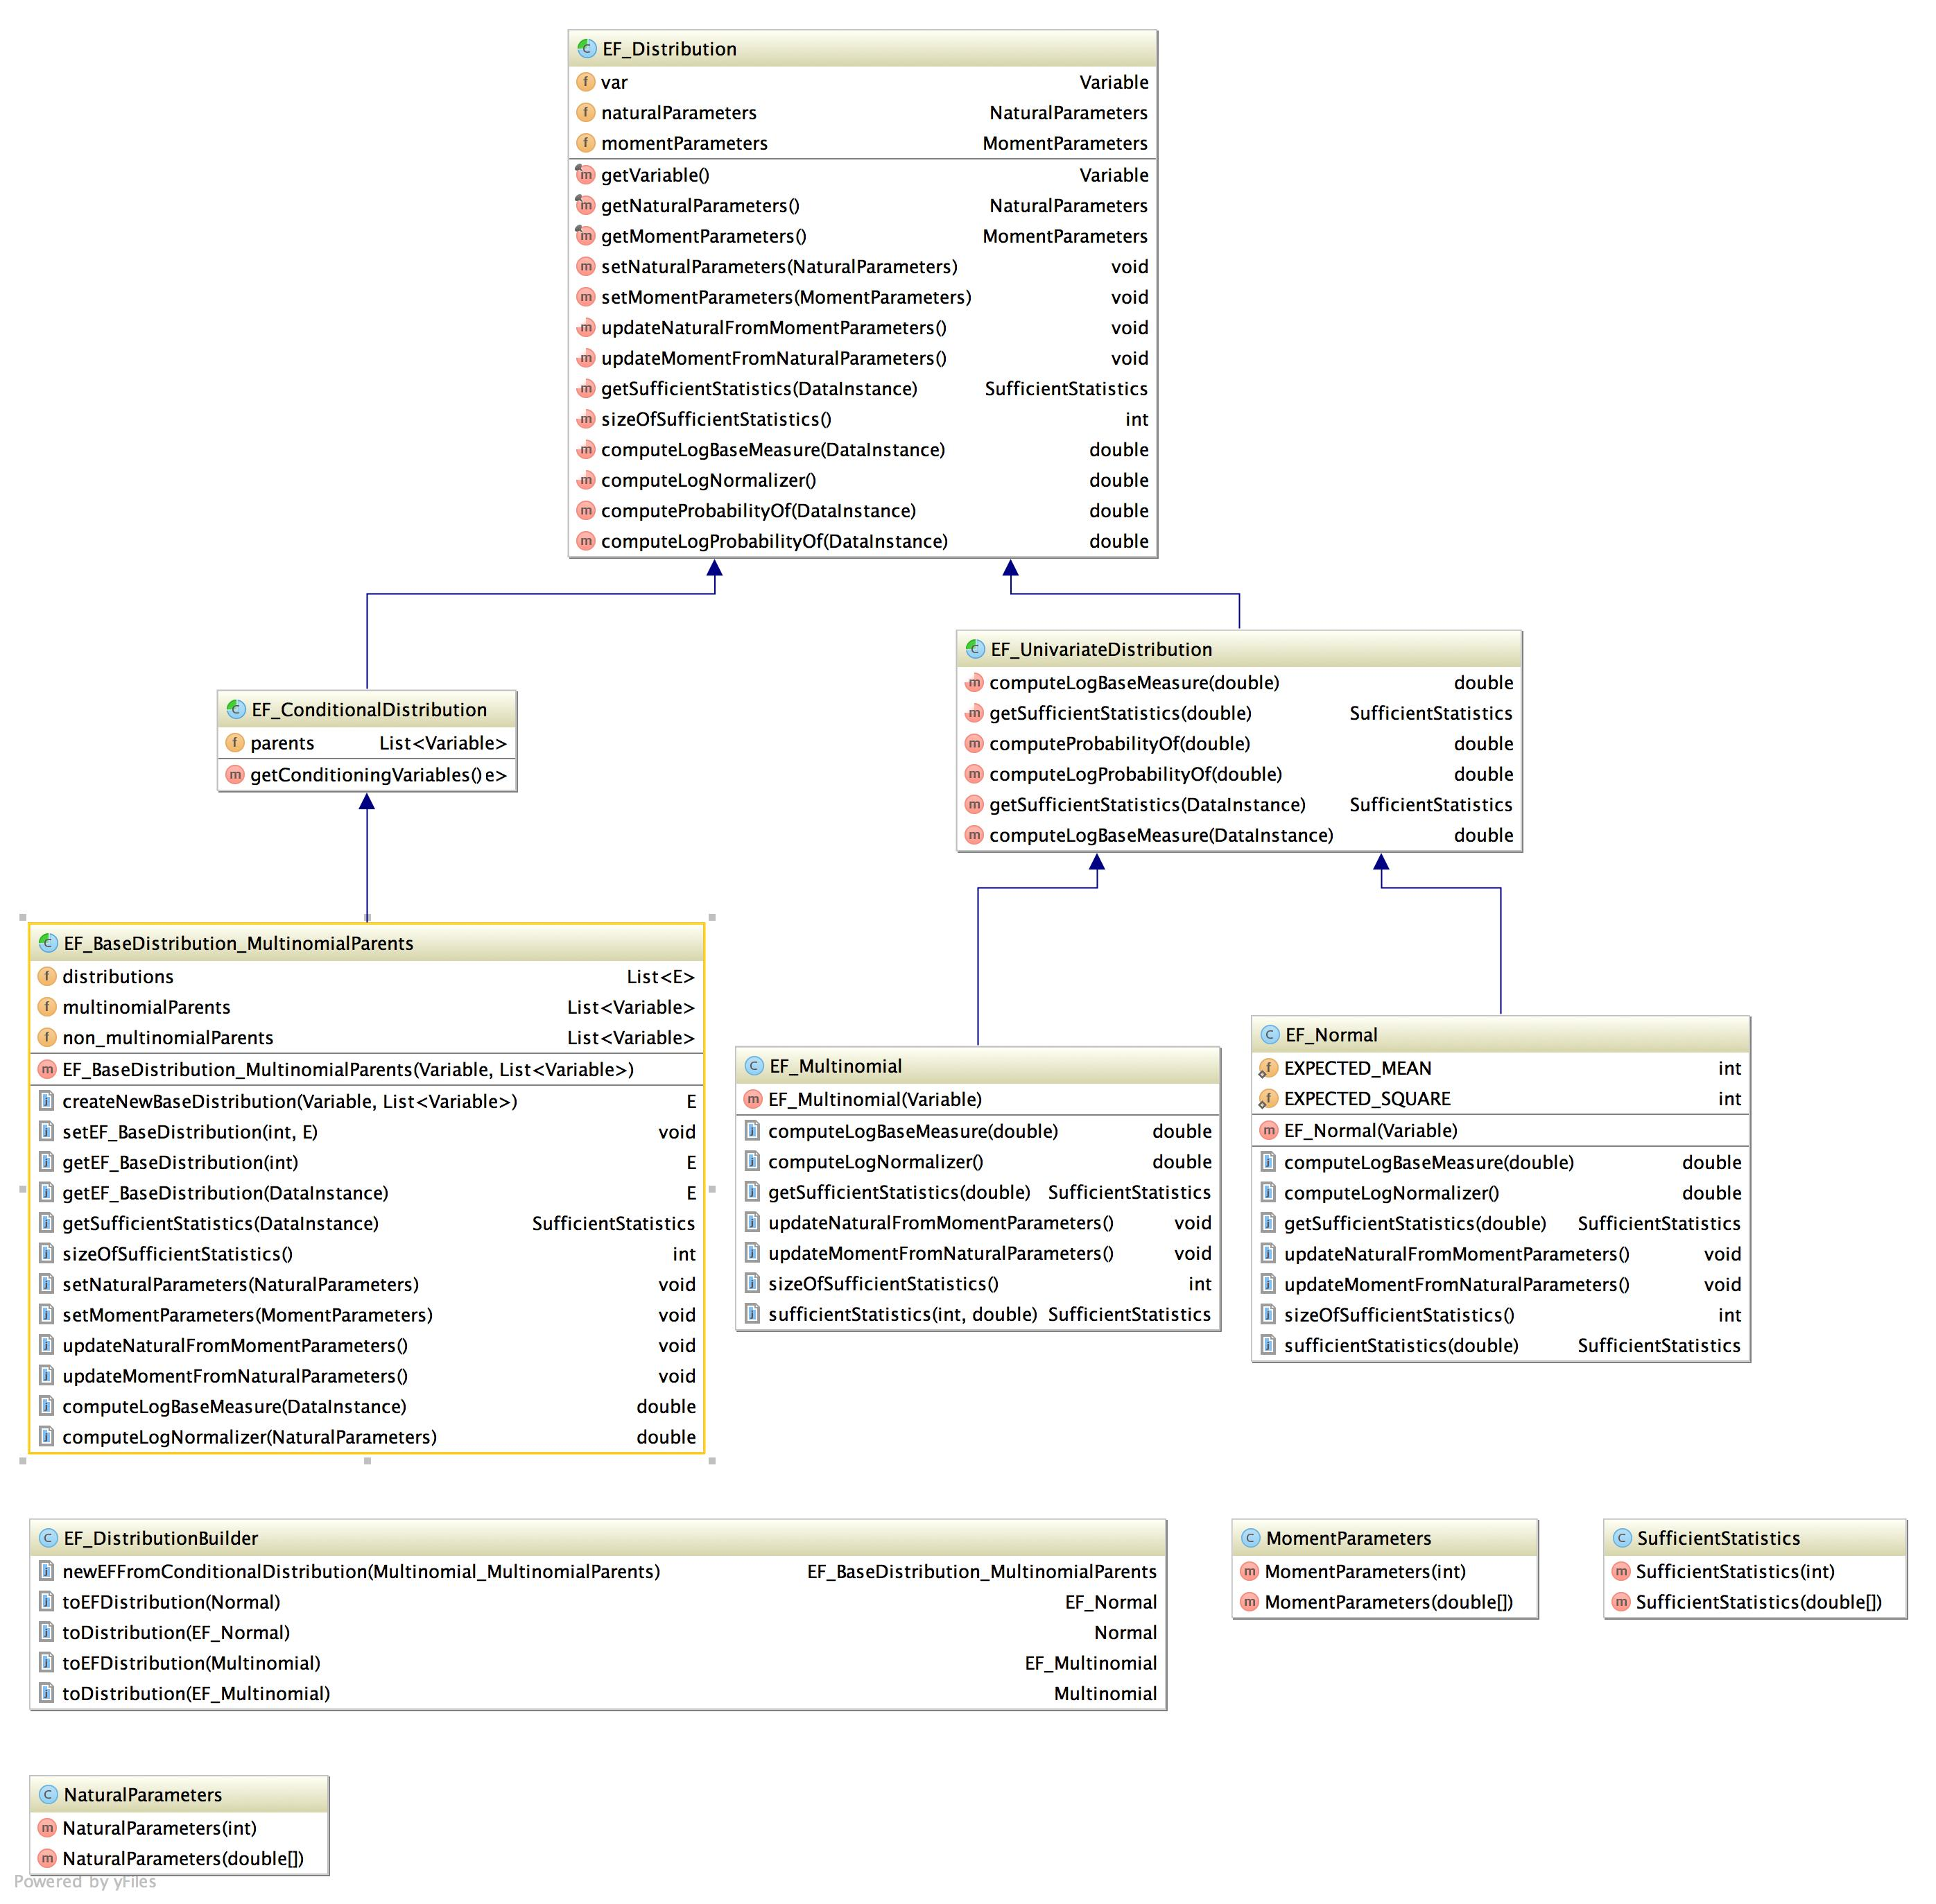
\includegraphics[width=\textwidth]{ClassDiagrams/core_exponentialfamily.jpg}
\end{figure}

\subsection{Package core.exponentialfamily}
\begin{figure}[H]
  %\caption{Class diagram of the package: \texttt{core.huginlink}}
  \centering
    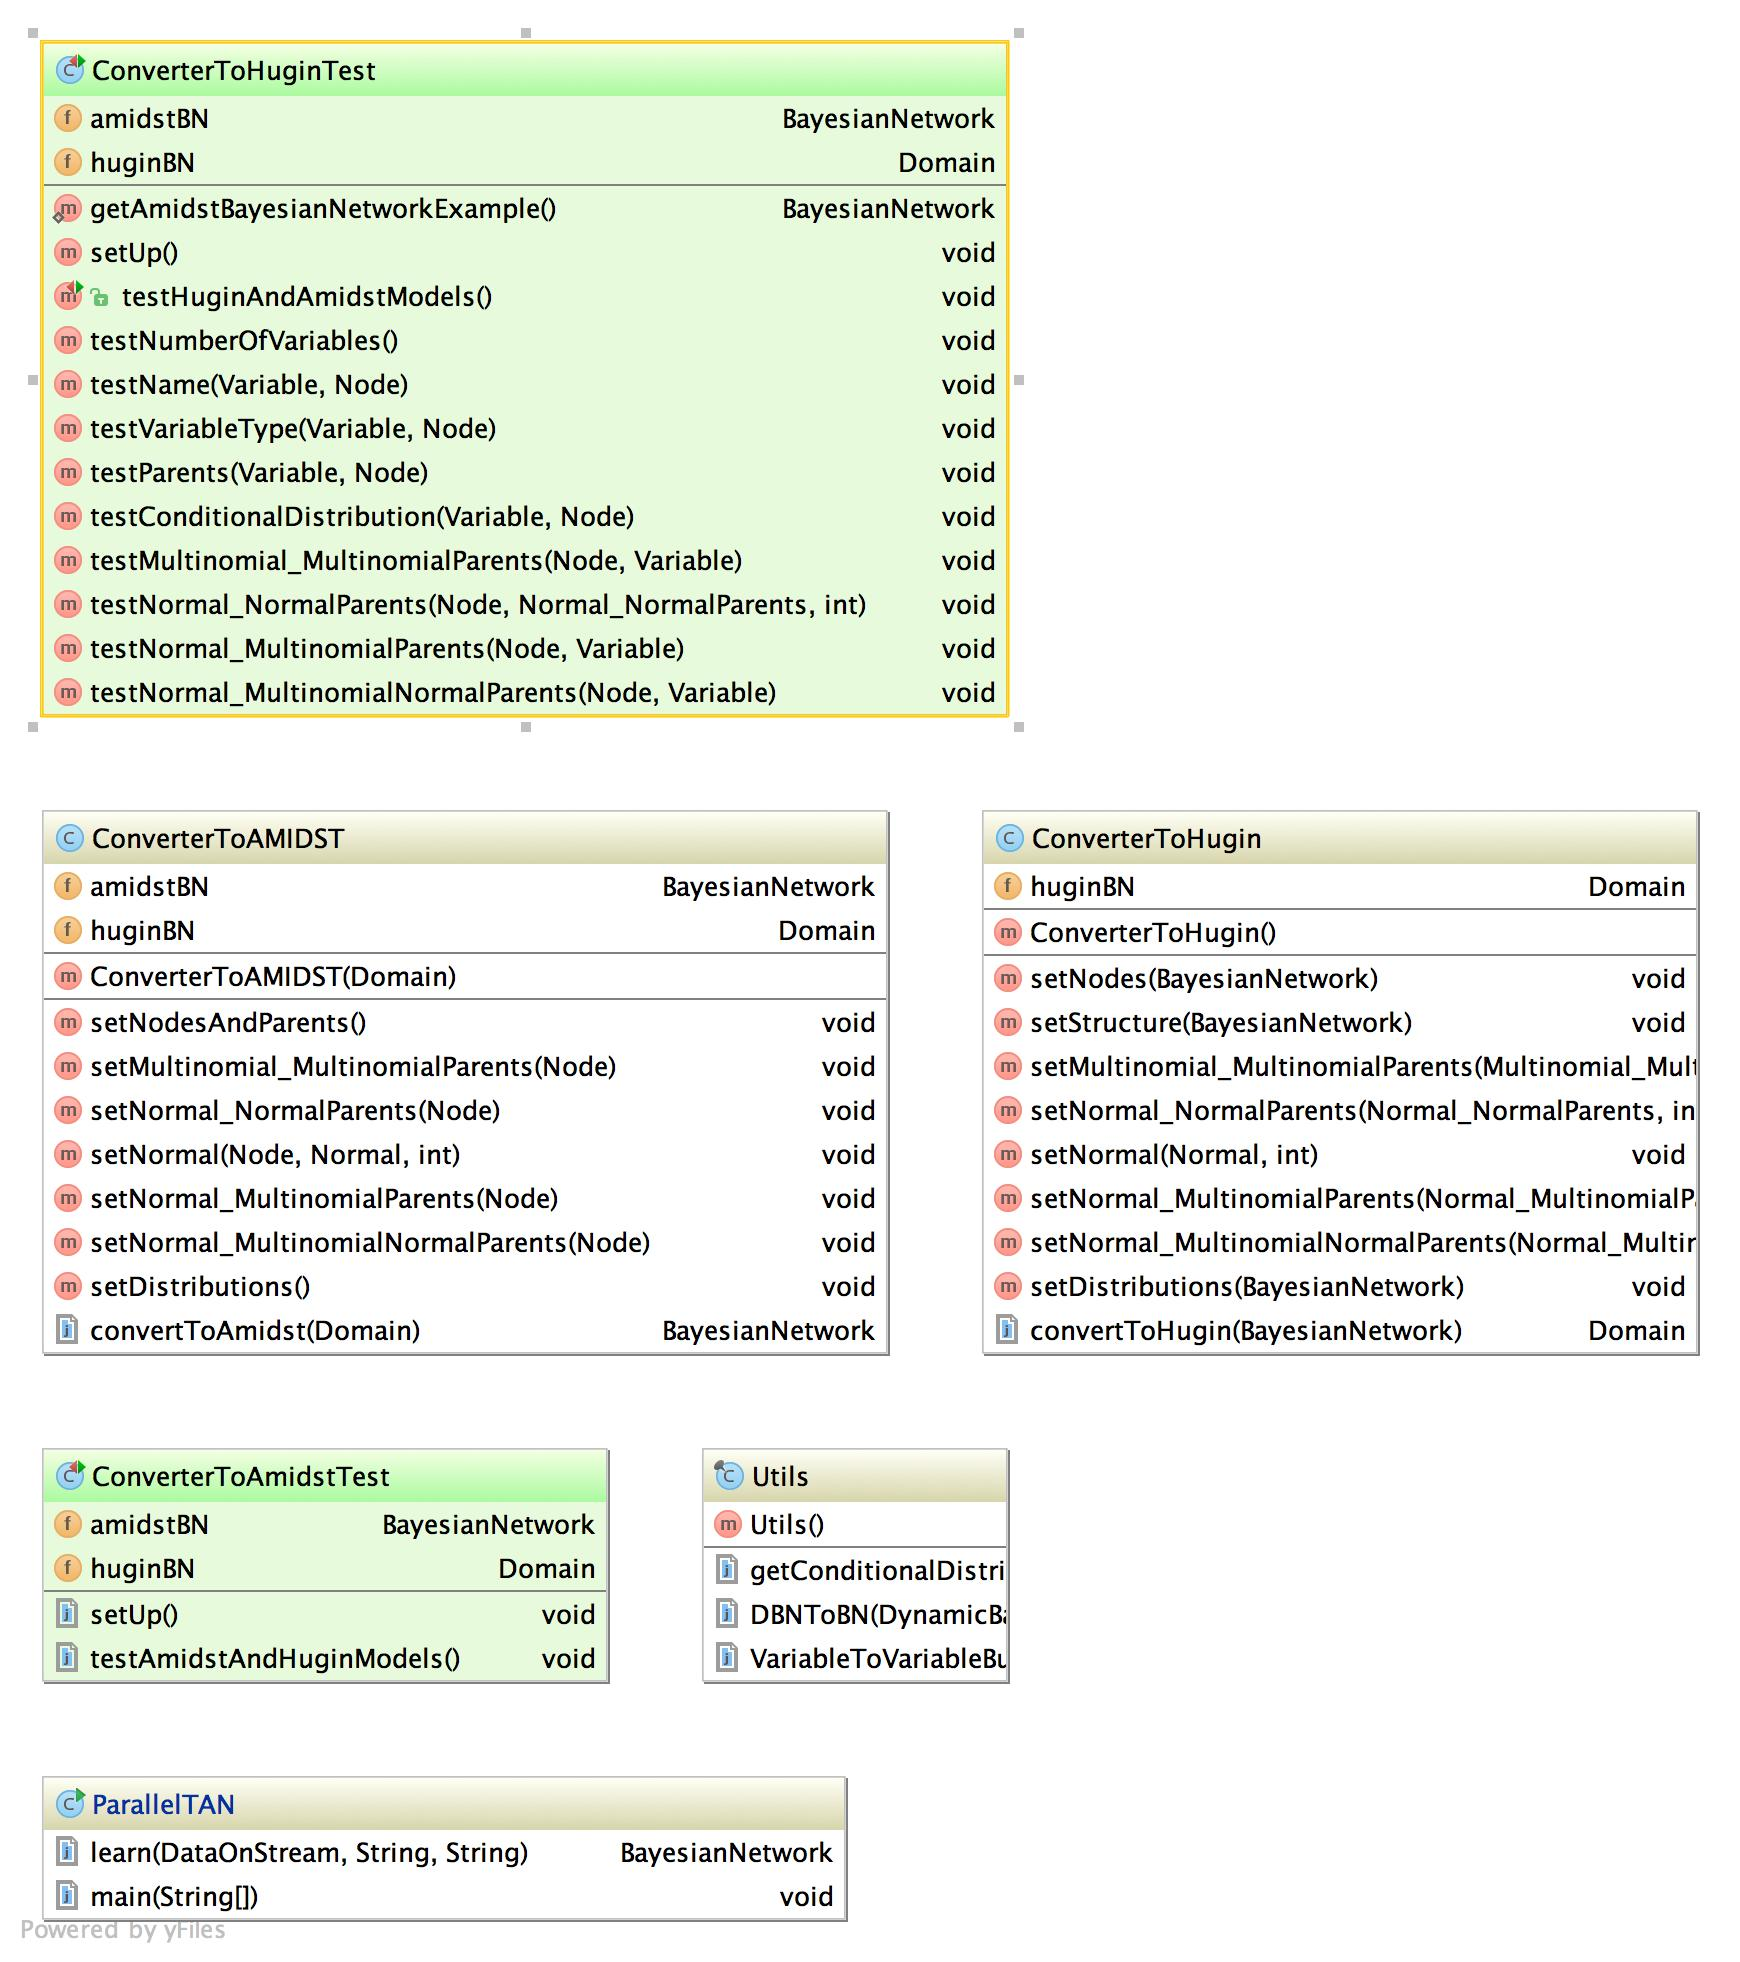
\includegraphics[width=0.7\textwidth]{ClassDiagrams/core_huginlink.jpg}
\end{figure}

\subsection{Package core.modelstructure}
\begin{figure}[H]
  %\caption{Class diagram of the package: \texttt{core.modelstructure}}
  \centering
    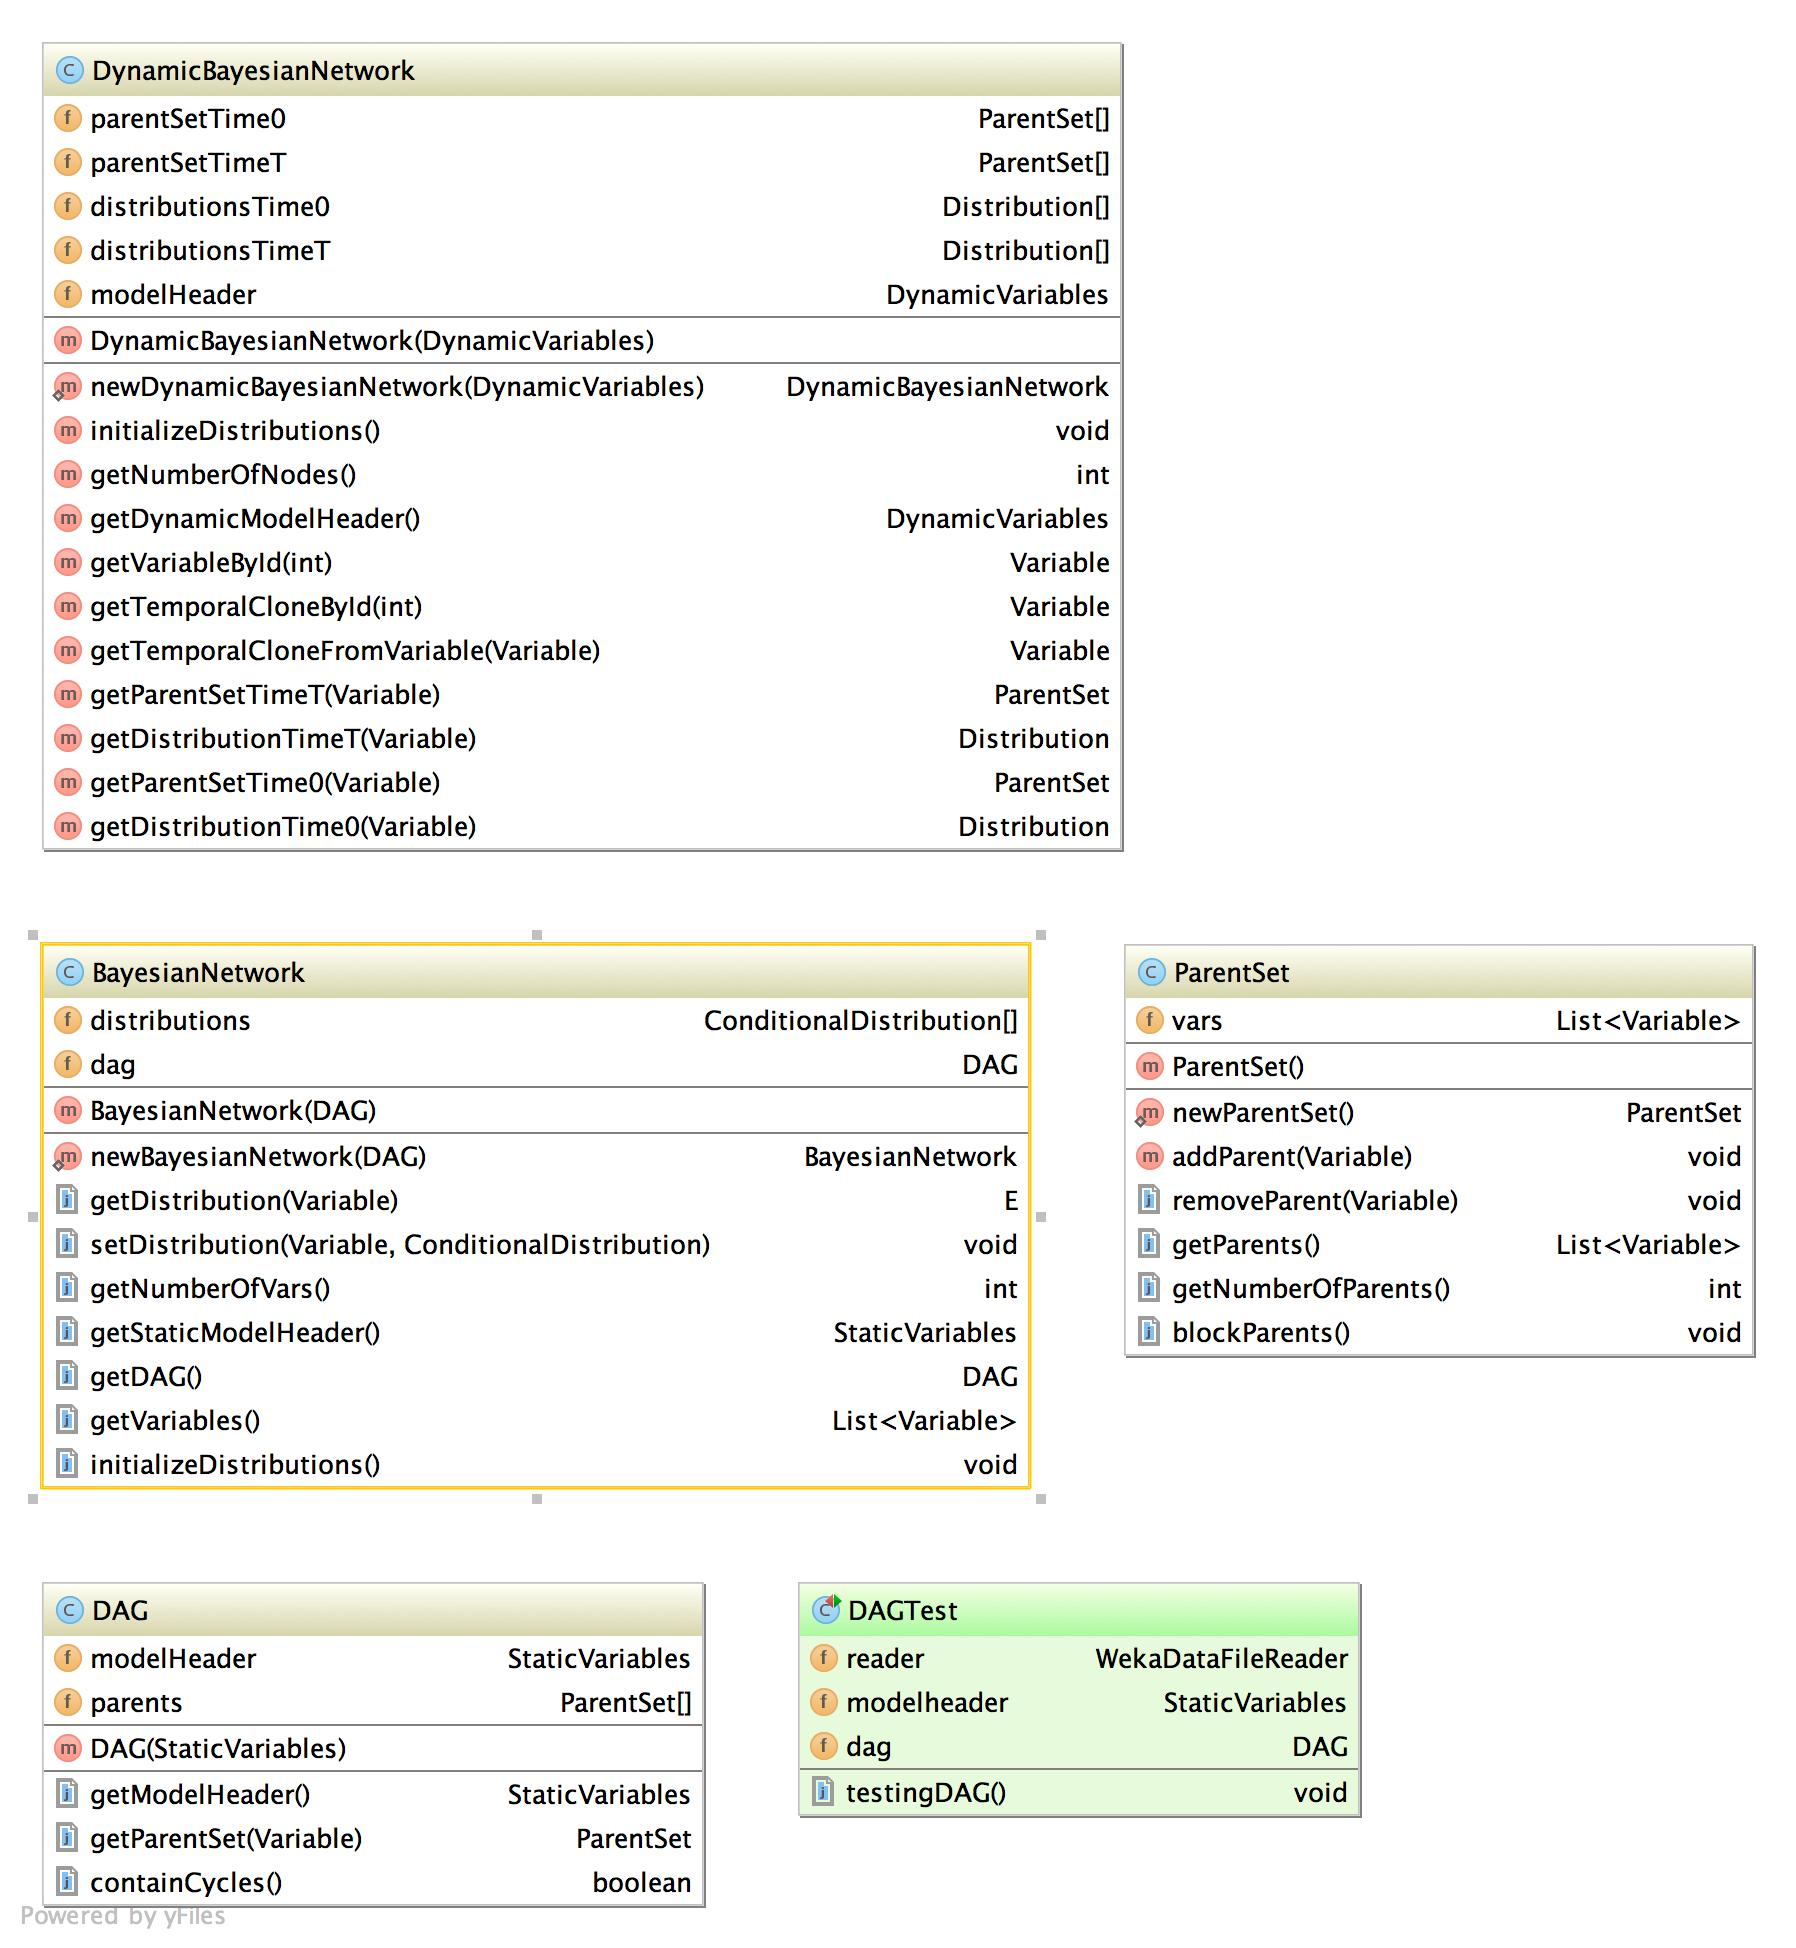
\includegraphics[width=\textwidth]{ClassDiagrams/core_modelstructure.jpg}
\end{figure}


\subsection{Package core.potential}
\begin{figure}[H]
  \caption{Class diagram of the package: \texttt{core.potential}}
  \centering
    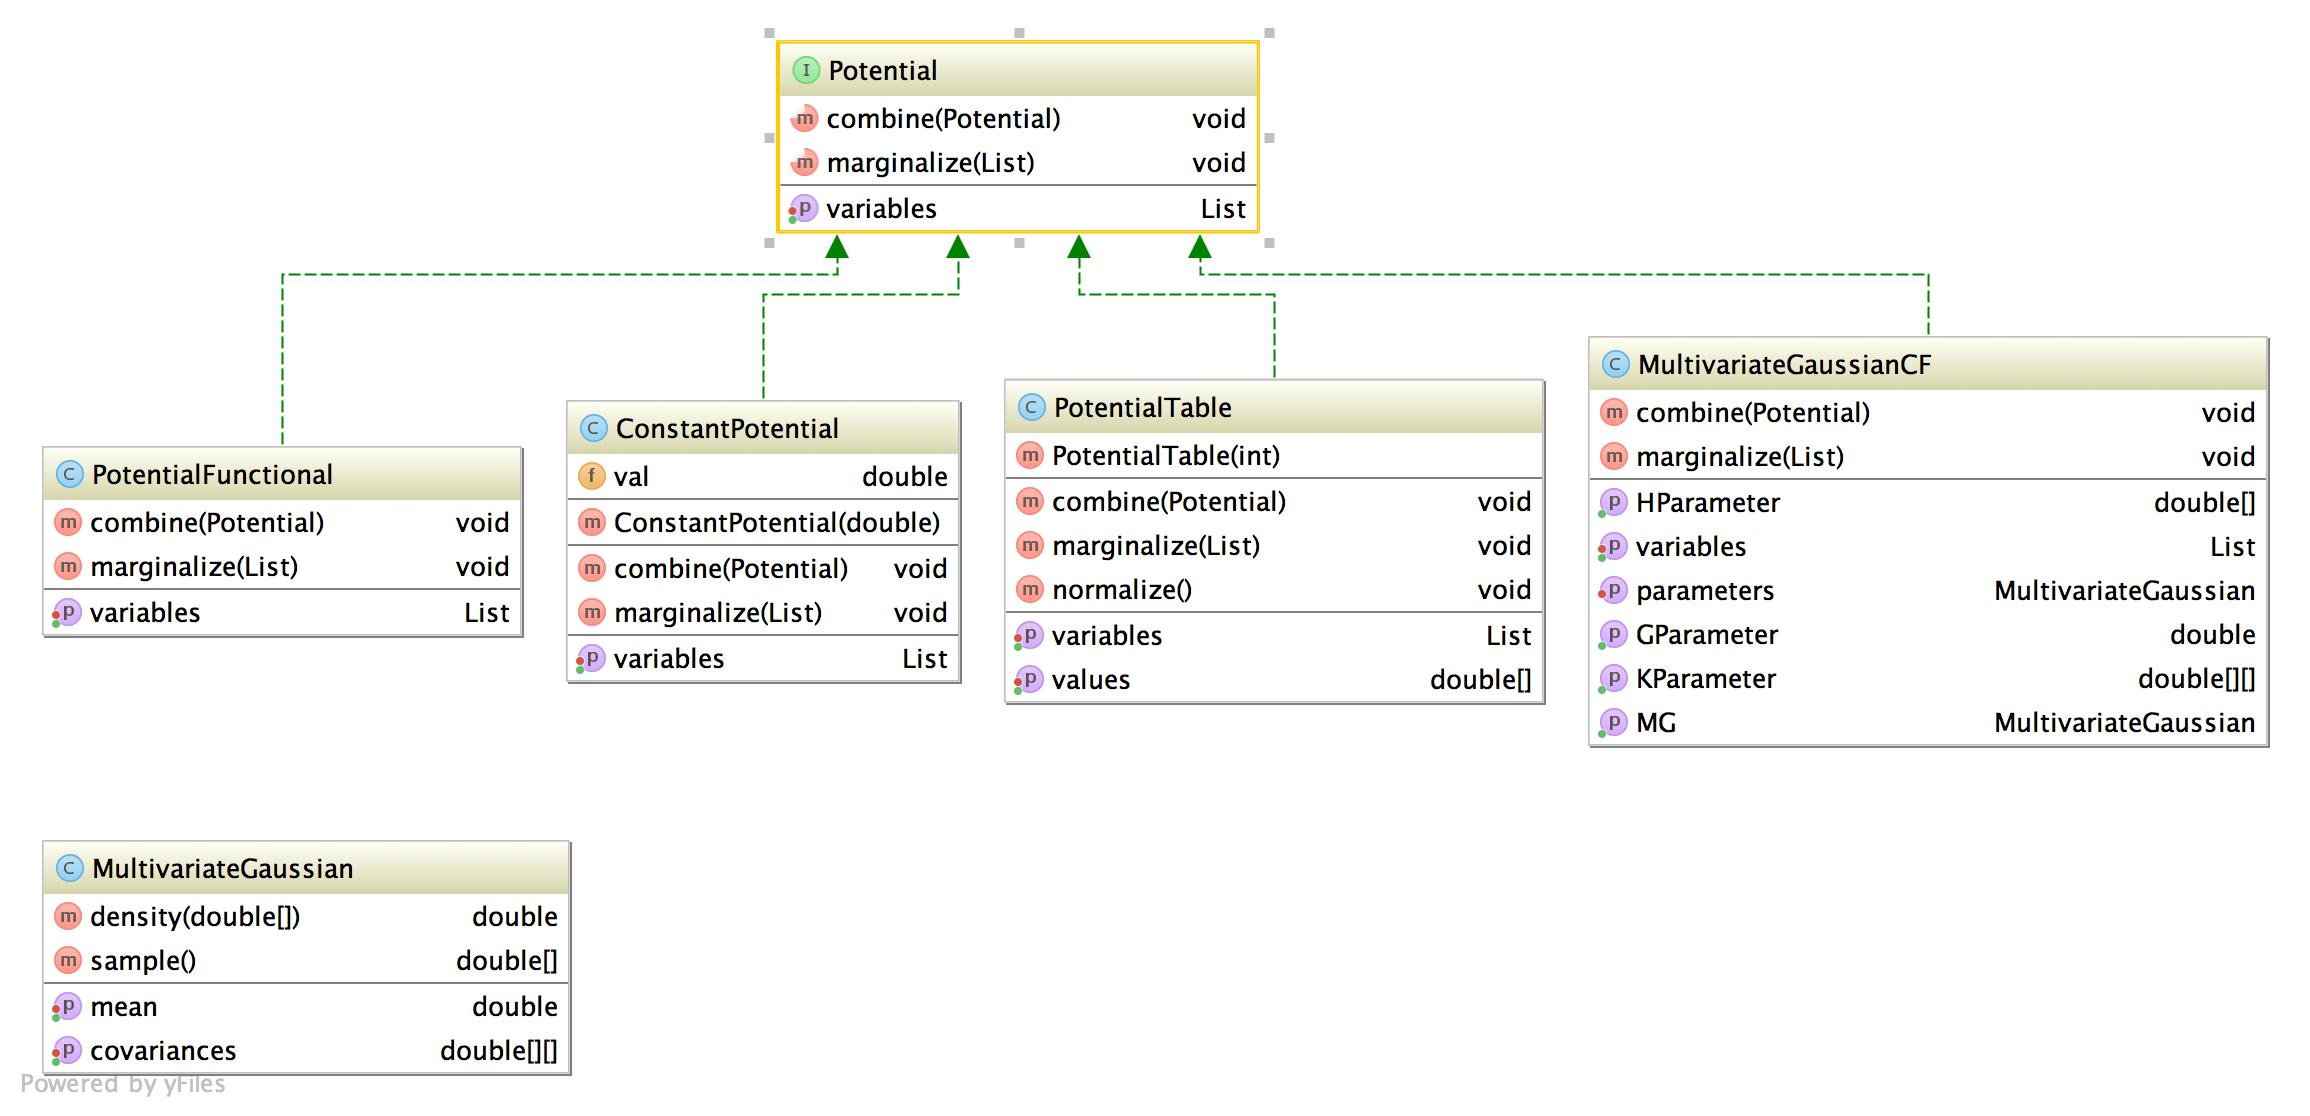
\includegraphics[width=\textwidth]{ClassDiagrams/core_potential.jpg}
\end{figure}

\subsection{Package core.utils}
\begin{figure}[H]
  %\caption{Class diagram of the package: \texttt{core.utils}}
  \centering
    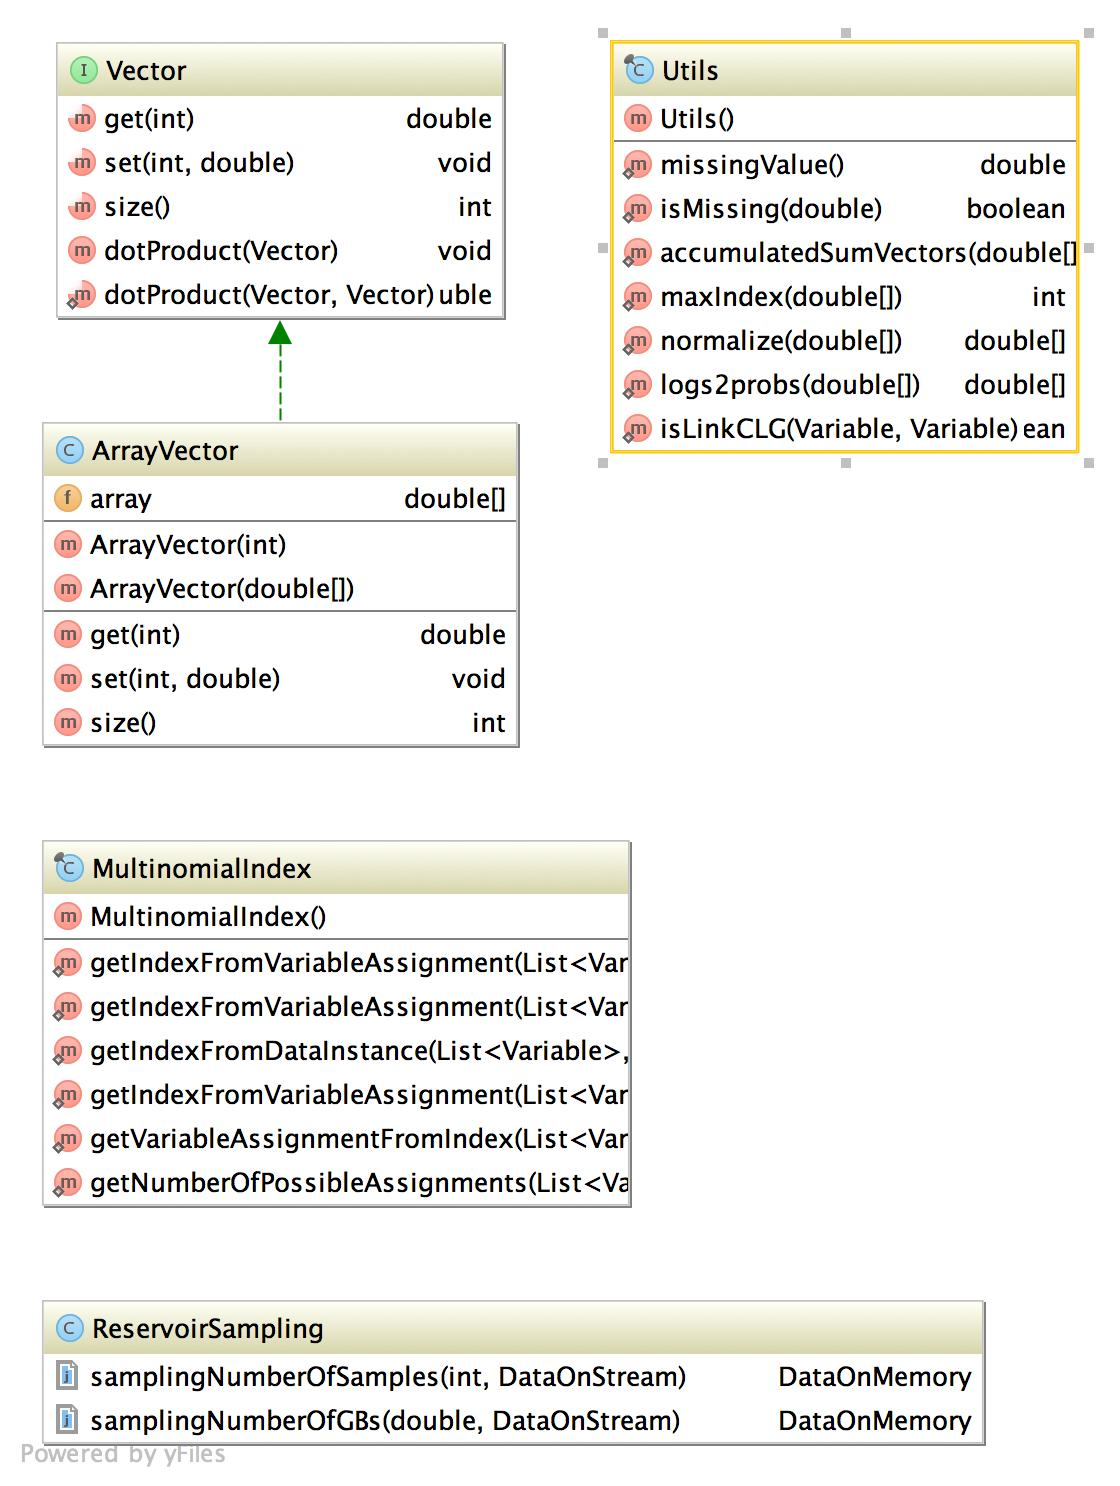
\includegraphics[width=0.6\textwidth]{ClassDiagrams/core_utils.jpg}
\end{figure}


\subsection{Package core.variables}
\begin{figure}[H]
  \caption{Class diagram of the package: \texttt{core.variables}}
  \centering
    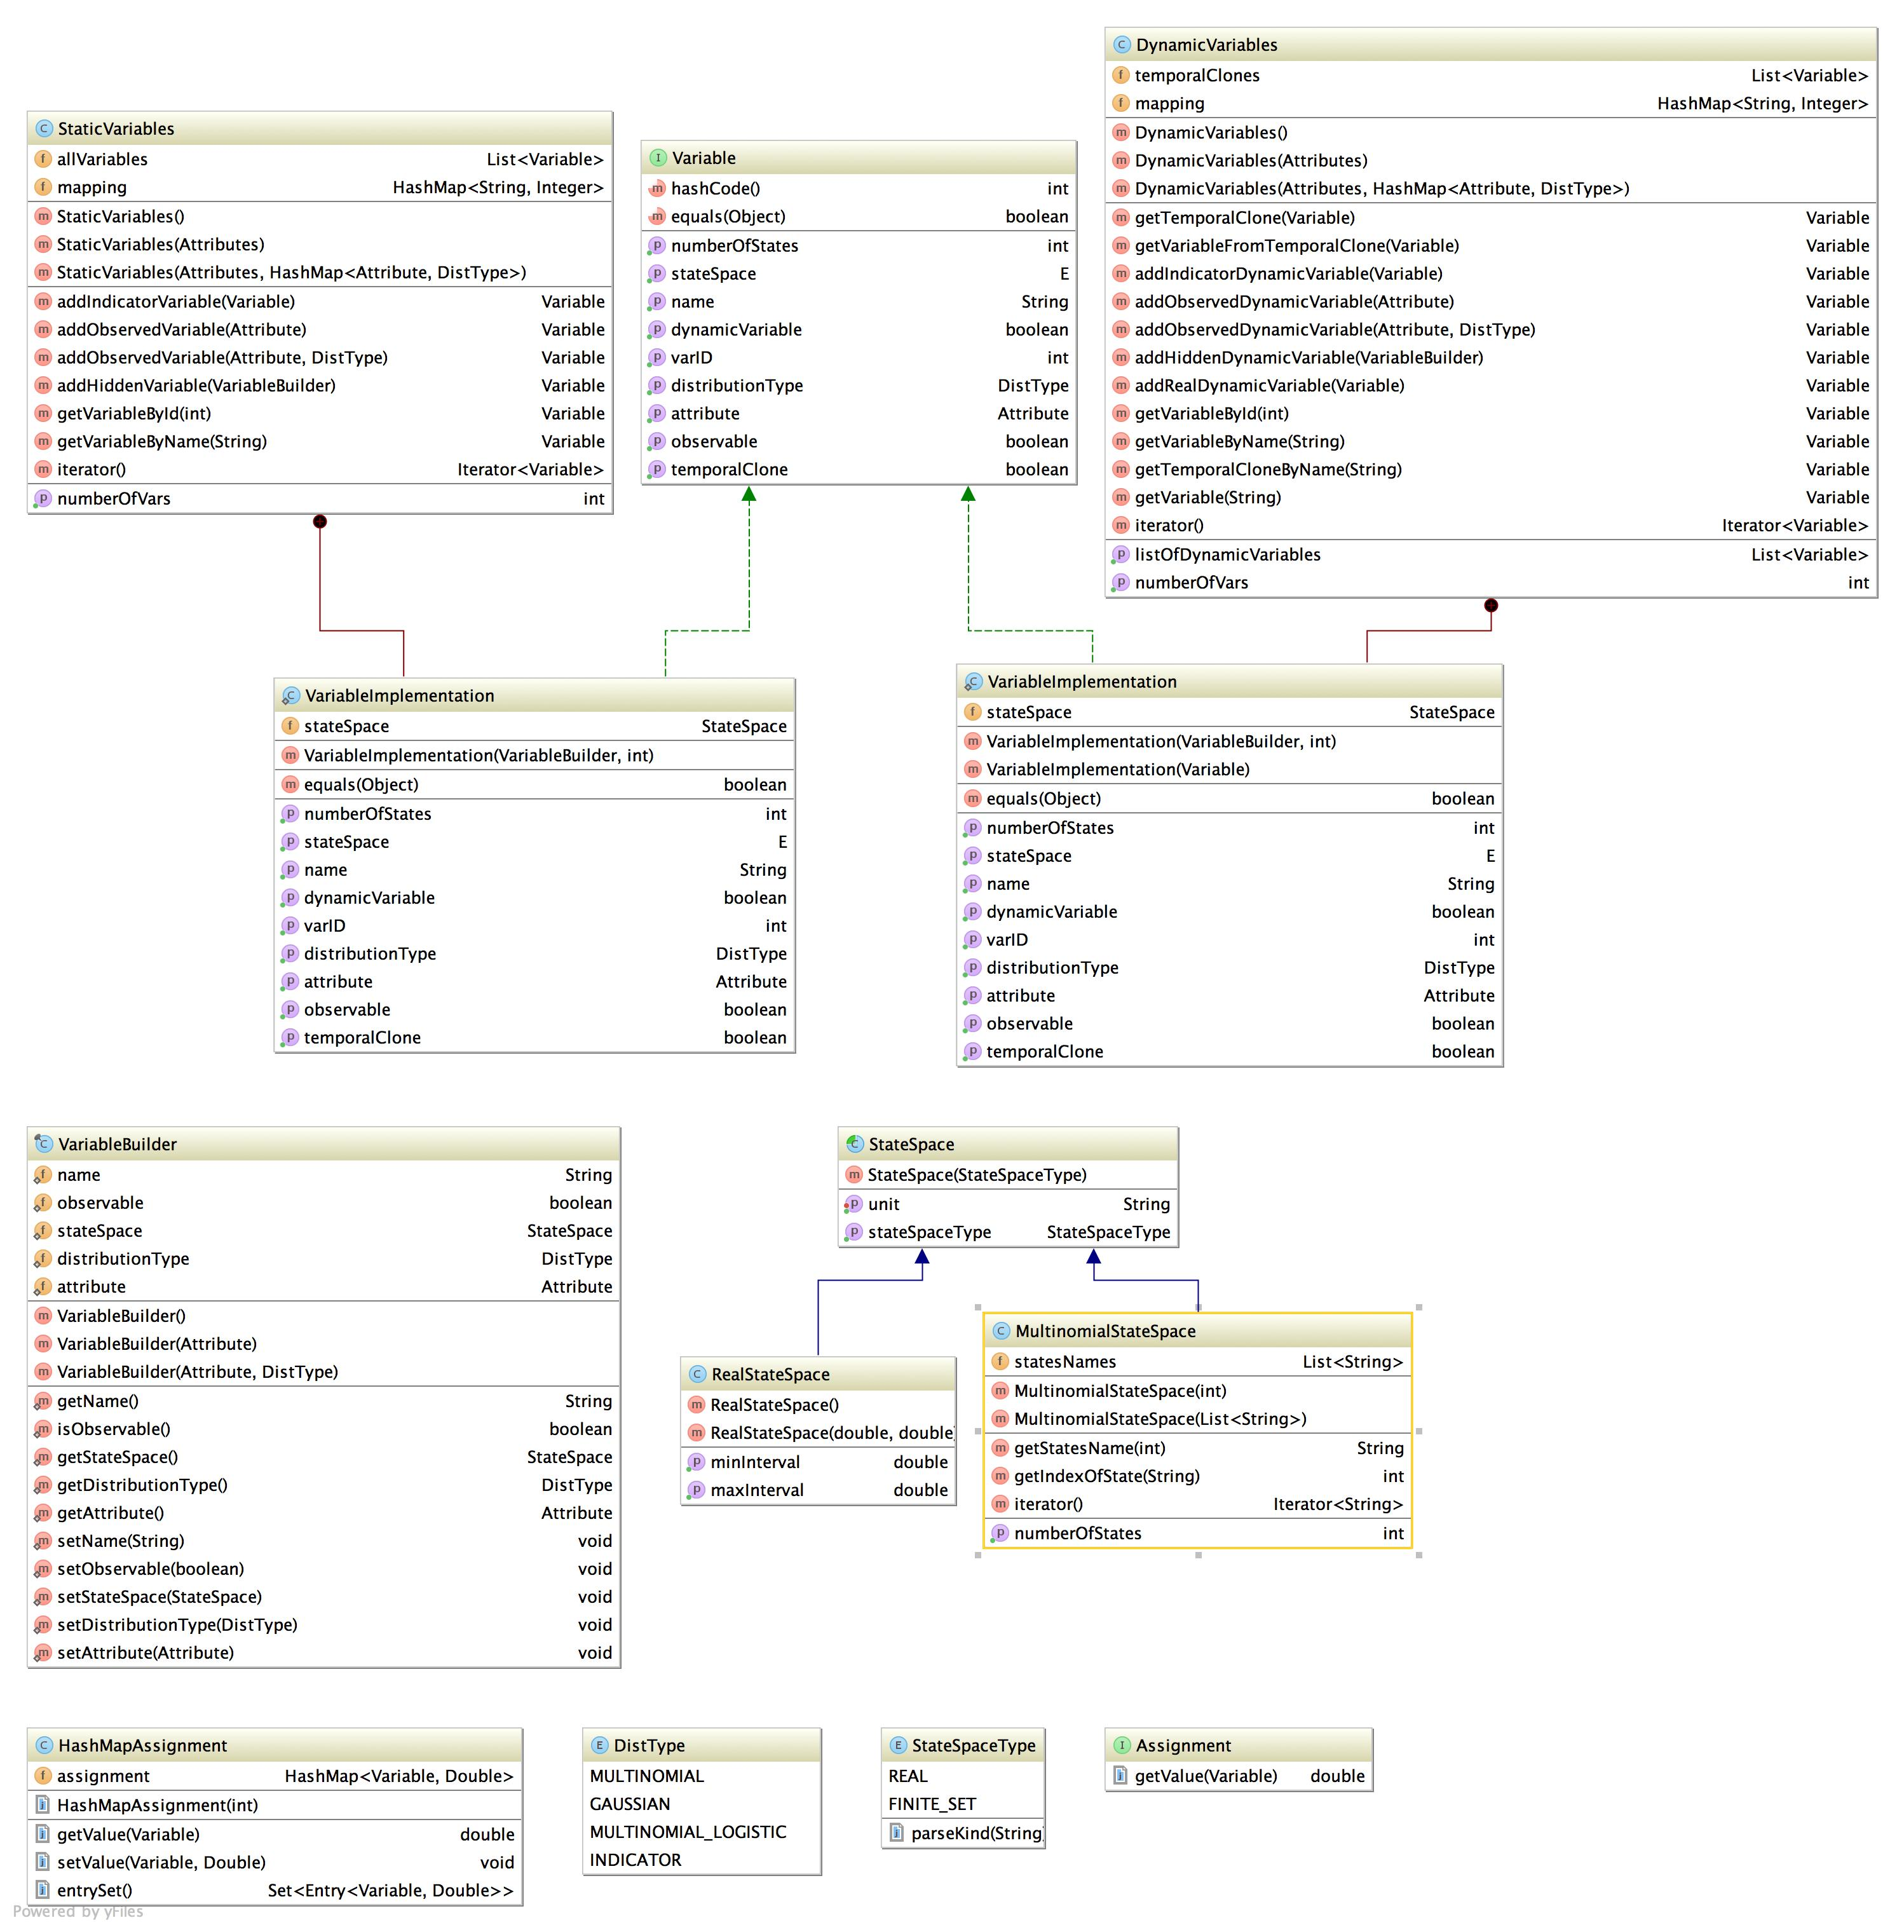
\includegraphics[width=\textwidth]{ClassDiagrams/core_variables.jpg}
\end{figure}

